\documentclass[12pt]{article}
\usepackage[T2A]{fontenc}
\usepackage[utf8]{inputenc}
\usepackage{multirow}
\usepackage{caption}
\usepackage{subcaption}
\usepackage{amsmath}
\usepackage{changepage}
\usepackage{graphicx}
\usepackage{float}
\usepackage[english,russian]{babel}
\usepackage{amsmath, amsfonts, amssymb, amsthm, mathtools}
\usepackage{xcolor}
\usepackage{array}
\usepackage{hyperref}
\usepackage[top = 1.5cm, left = 1.5 cm, right = 1.5 cm, bottom = 3 cm]{geometry}
\graphicspath{ {./figures/} }
  
\begin{document}
\begin{titlepage}
    \begin{center}
        {\large МОСКОВСКИЙ ФИЗИКО-ТЕХНИЧЕСКИЙ ИНСТИТУТ (НАЦИОНАЛЬНЫЙ ИССЛЕДОВАТЕЛЬСКИЙ УНИВЕРСИТЕТ)}
    \end{center}
    \begin{center}
        {\large Физтех-школа физики и исследований им. Ландау}
    \end{center}
    
    
    \vspace{3cm}
    {\huge
        \begin{center}
            \textbf{Определение силы Архимеда, действующей на отдельные молекулы слабо-неидеального газа во внешнем поле.}
        \end{center}
    }
    \vspace{2cm}
    \begin{flushright}
        {\LARGE Автор:\\ Шахматов Андрей Юрьевич \\
            \vspace{0.2cm}
            Б02-304}
    \end{flushright}
    \vspace{7 cm}
    \begin{center}
        Долгопрудный 2024
    \end{center}
\end{titlepage}

% \maketitle

\begin{abstract}
    Рассмотрен вопрос действия силы Архимеда на отдельные молекулы 
    вещества. Предложена причина возникновения силы Архимеда для одиночных молекул. 
    Рассчитана сила Архимеда для слабо-неидеальных веществ, при этом рассмотрены 
    случаи атомарного вещества и плазмы. Определено, что характерным параметром, 
    определяющим силу Архимеда для атомарного вещества является 
    второй вириальный коэффициент.
\end{abstract}

\tableofcontents

\section{Введение}
Основопологающим законом гидростатики безусловно является закон Архимеда, для макроскопических тел его 
формулировка звучит так: на тело, погружённое в жидкость или газ, действует выталкивающая сила, 
численно равная весу объёма жидкости или газа, вытесненного телом. Однако возникает вопрос, можно ли считать 
телом, погружённым в вещество, одну из молекул данного вещества. Согласно оригинальной формулировке 
закона Архимеда, до тех пор пока объём рассматриваемого тела много больше объёма частицы вещества справедливо 
следующее выражение
\begin{equation}
    F_{a} = -\rho g V_0. 
    \label{eq:1}
\end{equation}
Легко понять, что для отдельной молекулы силв Архимеда может неравняться нулю. Данный 
факт легко проверить рассмотрев поведение молекулы несжимаемой жидкости. На каждую молекулу 
жидкости действует сила тяжести, однако молекула не падает, что означает наличие силы противонаправленной 
силе тяжести - силы Архимеда. Также стоит отметить несостоятельность формулы \ref{eq:1} для описания данного 
случая, так как плотность молекулы больше плотности жидкости в общем (между молекулами в жидкости есть 
пустоты), тогда согласно формуле \ref{eq:1} молекула должна тонуть.
Для объяснения несогласованности можно привести следующую качественную модель: вокруг молекулы в жидкости 
находится некоторый объём, в который не могут попасть другие молекулы, в таком случае "эффективный" объём 
молекулы $V_0$, использующийся в формуле \ref{eq:1} складывается из собственного объёма молекулы $V$ и присоединённой 
пустой части - "недоступного объёма" $V^{\prime}$ . В таком случае сила Архимеда оказывается равна: 
\begin{equation}
    F_a = -\rho g (V + V^{\prime}).
    \label{eq:2}
\end{equation}

\section{Расчёт силы Архимеда для слабо-неидеальных газов}
Перейдём к количественному выводу силы Архимеда, действующей на слабо-неидеальные газы. Такие газы 
делятся на два принципиально различных класса: атомарные и плазменные. В случае атомарных газов 
взаимодействие между молекулами быстро спадает с расстоянием $U \propto \frac{1}{r^6}$ и потому можно считать 
взаимодействие между далёкими молекулами нулевым. Однако в случае плазменных газов потенциал взаимодействия 
является кулоновским $U \propto \frac{1}{r}$ и слишком слабо спадает с расстоянием, в таком случае пренебрегать 
взаимодействием с более далёкими молекулами нельзя. Отдельно рассмотрим два типа газов. 
\subsection*{Атомарные слабо-неидеальные газы}
Выражение для свободной энергии для атомарных газов можно приблизить вириальным разложением (Приложение \ref{app:1}), 
в нашей работе ограничимся двумя членами разложения: 
\begin{equation}
    F = F_0 + \frac{N^{2}kT}{V} b(T),
    \label{eq:3}
\end{equation} 
где $F_0$ - свободная энергия идеального газа, $b(T)$ - второй Вириальный коэффициент: 
\begin{equation}
    b(T) = \frac{1}{2} \int \left( 1 - \exp \left\{ -\frac{U(r)}{kT} \right\}  \right)  \,\mathrm{d}V,
    \label{eq:4}
\end{equation}  
где $U(r)$ - энергия взаимодействия между двумя молекулами. 
Свободная энергия идеального газа $F_0$ выражается как 
\begin{equation}
    F_0 = NkT \ln \frac{N}{V} - N h(T), 
    \label{eq:5}
\end{equation} 
где $h(T)$ - некоторая функция температуры. 
Также запишем выражение для химического потенциала $\mu$  атомарного газа 
\begin{equation}
    \mu = \left( \frac{\partial F}{\partial N} \right)_{T, V} = kT \ln n + 2nkT b(T) - h(T).
    \label{eq:6}
\end{equation}
Перейдём к выводу непосредственно силы Архимеда. Условие равновесия молекулы устанавливается 
постоянством гравихимического потенциала $\overline{\mu}$ (Приложение \ref{app:2}):
\begin{equation}
    \overline{\mu} = \mu + mgz = const.
    \label{eq:7}
\end{equation}
Продифференцировав равенство получим: 
\begin{equation}
    \frac{kT}{n} \frac{dn}{dz} = -\left( mg + 2 \frac{dn}{dz} kT b(T) \right). 
    \label{eq:8}
\end{equation}
Подставив вместо концентрации $n$: 
\begin{equation}
    n(z) = n_0 \exp \left( \frac{-A(z)}{kT} \right), 
    \label{eq:9}
\end{equation} 
где $A(z)$ - работа силы по отношению к молекуле газа. Получим формулу для полной силы, действующей 
на молекулу: 
\begin{equation}
    F_p = \frac{dA(z)}{dz} = mg + 2 \frac{dn}{dz} kT b(T).
    \label{eq:10}
\end{equation} 
Слагаемое $mg$ очевидно отвечает за силу тяжести, действующуу на молекулу, тогда сила Архимеда вычисляется как 
\begin{equation}
    F_a = 2 \frac{dn}{dz} kT b(T).
    \label{eq:11}
\end{equation}
Продифференцировав свободную энергию найдём уравнение состояния: 
\begin{equation}
    P = nkT + n^2kTb(T).
    \label{eq:12}
\end{equation}
Тогда 
\[
    \frac{dP}{dz} \approx kT \frac{dn}{dz}.
\]
Подставляя полученный результат для концентраций в \ref{eq:11} получим 
\begin{equation}
    F_a = 2b(T) \frac{dP}{dz}.
    \label{eq:13}
\end{equation}
Перепишем полученную формулу через плотность с учётом $\frac{dP}{dz} = \rho g$, чтобы свести к стандартному виду закона Архимеда: 
\begin{equation}
    F_a = -2b(T)\rho g.
    \label{eq:14}
\end{equation}
Из полученной форулы можно воспринимать параметр $2b(T)$ - как эффективный объём молекулы. 
Заметим, что на молекулы идеального газа не действует силы Архимеда, так как вириальный коэффициент равен 0. 
Рассмотрим как выглядит сила Архимеда в случае неидеального газа, описывающегося 
моделью газа Ван-дер-Ваальса 
\begin{equation}
    b(T) = b - \frac{a}{T}.
    \label{eq:15}
\end{equation}
Тогда соответственно при $T = \frac{a}{b}$ - температура Бойля, сила Архимеда должна равняться нулю, а газ вести себя как идеальный. 
При больших температурах, $T \gg \frac{a}{b}$ $b(T) \approx b$, то есть взаимодействие между молекулами 
почти не оказывает влияния на силу Архимеда и газ описывается моделью упругих шариков.   
\subsection*{Классическая плазма}
В случае плазмы взаимодействие между ионами определяется кулоновским взаимодействием 
\[
    U = \frac{e^2}{r}
\] 
Для такого вещества нельзя пренебрегать непарными взаимодействиями, и потому не выполняется вириальное
разложение \ref{eq:3}. В таком случае применяется подход, основанный на усреднении полей (Приложение \ref{app:3}). 
Тогда свободная энергия может быть выражена как 
\begin{equation}
    F = F_0 - \frac{2e^3}{3} \sqrt{\frac{\pi N^3}{kTV}}\left( \sum_{i=1} n_i z_i \right)^\frac{3}{2}, 
    \label{eq:16}
\end{equation}
где $z_i$ - зарядовое число соответствующего иона, $n_i = \frac{N_i}{N}$ - количественная концентрация 
ионов с соответствующим зарядовым числом. Снова вычислим химический потенциал $\mu$
\begin{equation}
    \mu = \left( \frac{\partial F}{\partial N} \right)_{T, V} = kT \ln n - h(T) - e^3 \sqrt{\frac{\pi N}{kTV}}\left( \sum_{i=1} n_i z_i \right)^\frac{3}{2}.
    \label{eq:17}
\end{equation}   
Далее получим выражение, аналогичное \ref{eq:8}
\begin{equation}
    \frac{kT}{n} \frac{dn}{dz} = -\left( mg - \frac{e^3}{2} \sqrt{\frac{\pi}{kTn^3}} \frac{dn}{dz} \left( \sum_{i=1} n_i z_i \right)^\frac{3}{2} \right).
    \label{eq:18}
\end{equation}
После этого нетрудно выразить силу Архимеда
\begin{equation}
    F_a = -\frac{e^3}{2} \sqrt{\frac{\pi}{kTn^3}} \frac{dn}{dz} \left( \sum_{i=1} n_i z_i \right)^\frac{3}{2},
    \label{eq:19}
\end{equation}
знак минус означает, что сила Архимеда действует вверх. В отличие от атомарного газа, направление силы 
Архимеда не зависит от температуры, однако зависит от удельных концентраций зарядовых чисел $n_i z_i$. В случае 
большого количества отрицательно заряженных ионов сила Архимеда будет направлена противонаправленно с полем, 
а в случае большого количества положиетльно заряженных ионов сонаправленно. Также в случае плазмы сила 
Архимеда уже не будет пропорциональна разности давлений, как было в случае с атомарным газом \ref{eq:14}.
Стоит отметить, что при увеличении температуры сила модуль силы Архимеда у плазмы уменьшается, тогда как 
у атомарного газа увеличивается. 

\section{Симуляция}
Рассмотрена модель упругих шариков диаметра $d$. Моделирование проводилось для двумерного газа. 
В таком случае второй вириальный коэффициент вычисляется аналогично трёхмерному случаю и оказывается 
пропорционален диаметру в квадрате. Для проведения измерений сосуд делился на 12 секций и в каждой из 
них считалась концентрация молекул и средняя сила Архимеда. По полученным данным построены графики 
зависимости полной силы $F = F_A + F_g$ от концентрации $N$ (Рис. \ref{fig:FN}), за начало координат 
было положено значение силы тяжести $F_g = -0.2$. Из графиков видно, что 
зависимости хорошо аппроксимируются линейными зависимостями. Однако, в случае больших 
диаметров частиц линейные зависимости не проходят через начало координат, это может означать 
нарушение предложенной модели, так как между частицами происходит не только парное взаимодействие. 

Для каждого эксперимента были найдены коэффициенты наклона $k = \frac{\partial F}{\partial N}$, 
данные коэффициенты должны быть пропорциональны второму вириальному коэффициенту, а значит диаметру 
частицы в квадрате. Построен график зависимости $k$ от диаметра частицы $d^2$ (Рис. \ref{fig:kr}). 
Полученная зависимость может быть аппроксимирована прямой. При этом аппроксимирующая прямая 
пересекает начало координат, что подтверждается теорией (на идеальный газ сила Архимеда не действует).

\begin{figure}[H]
    \centering
    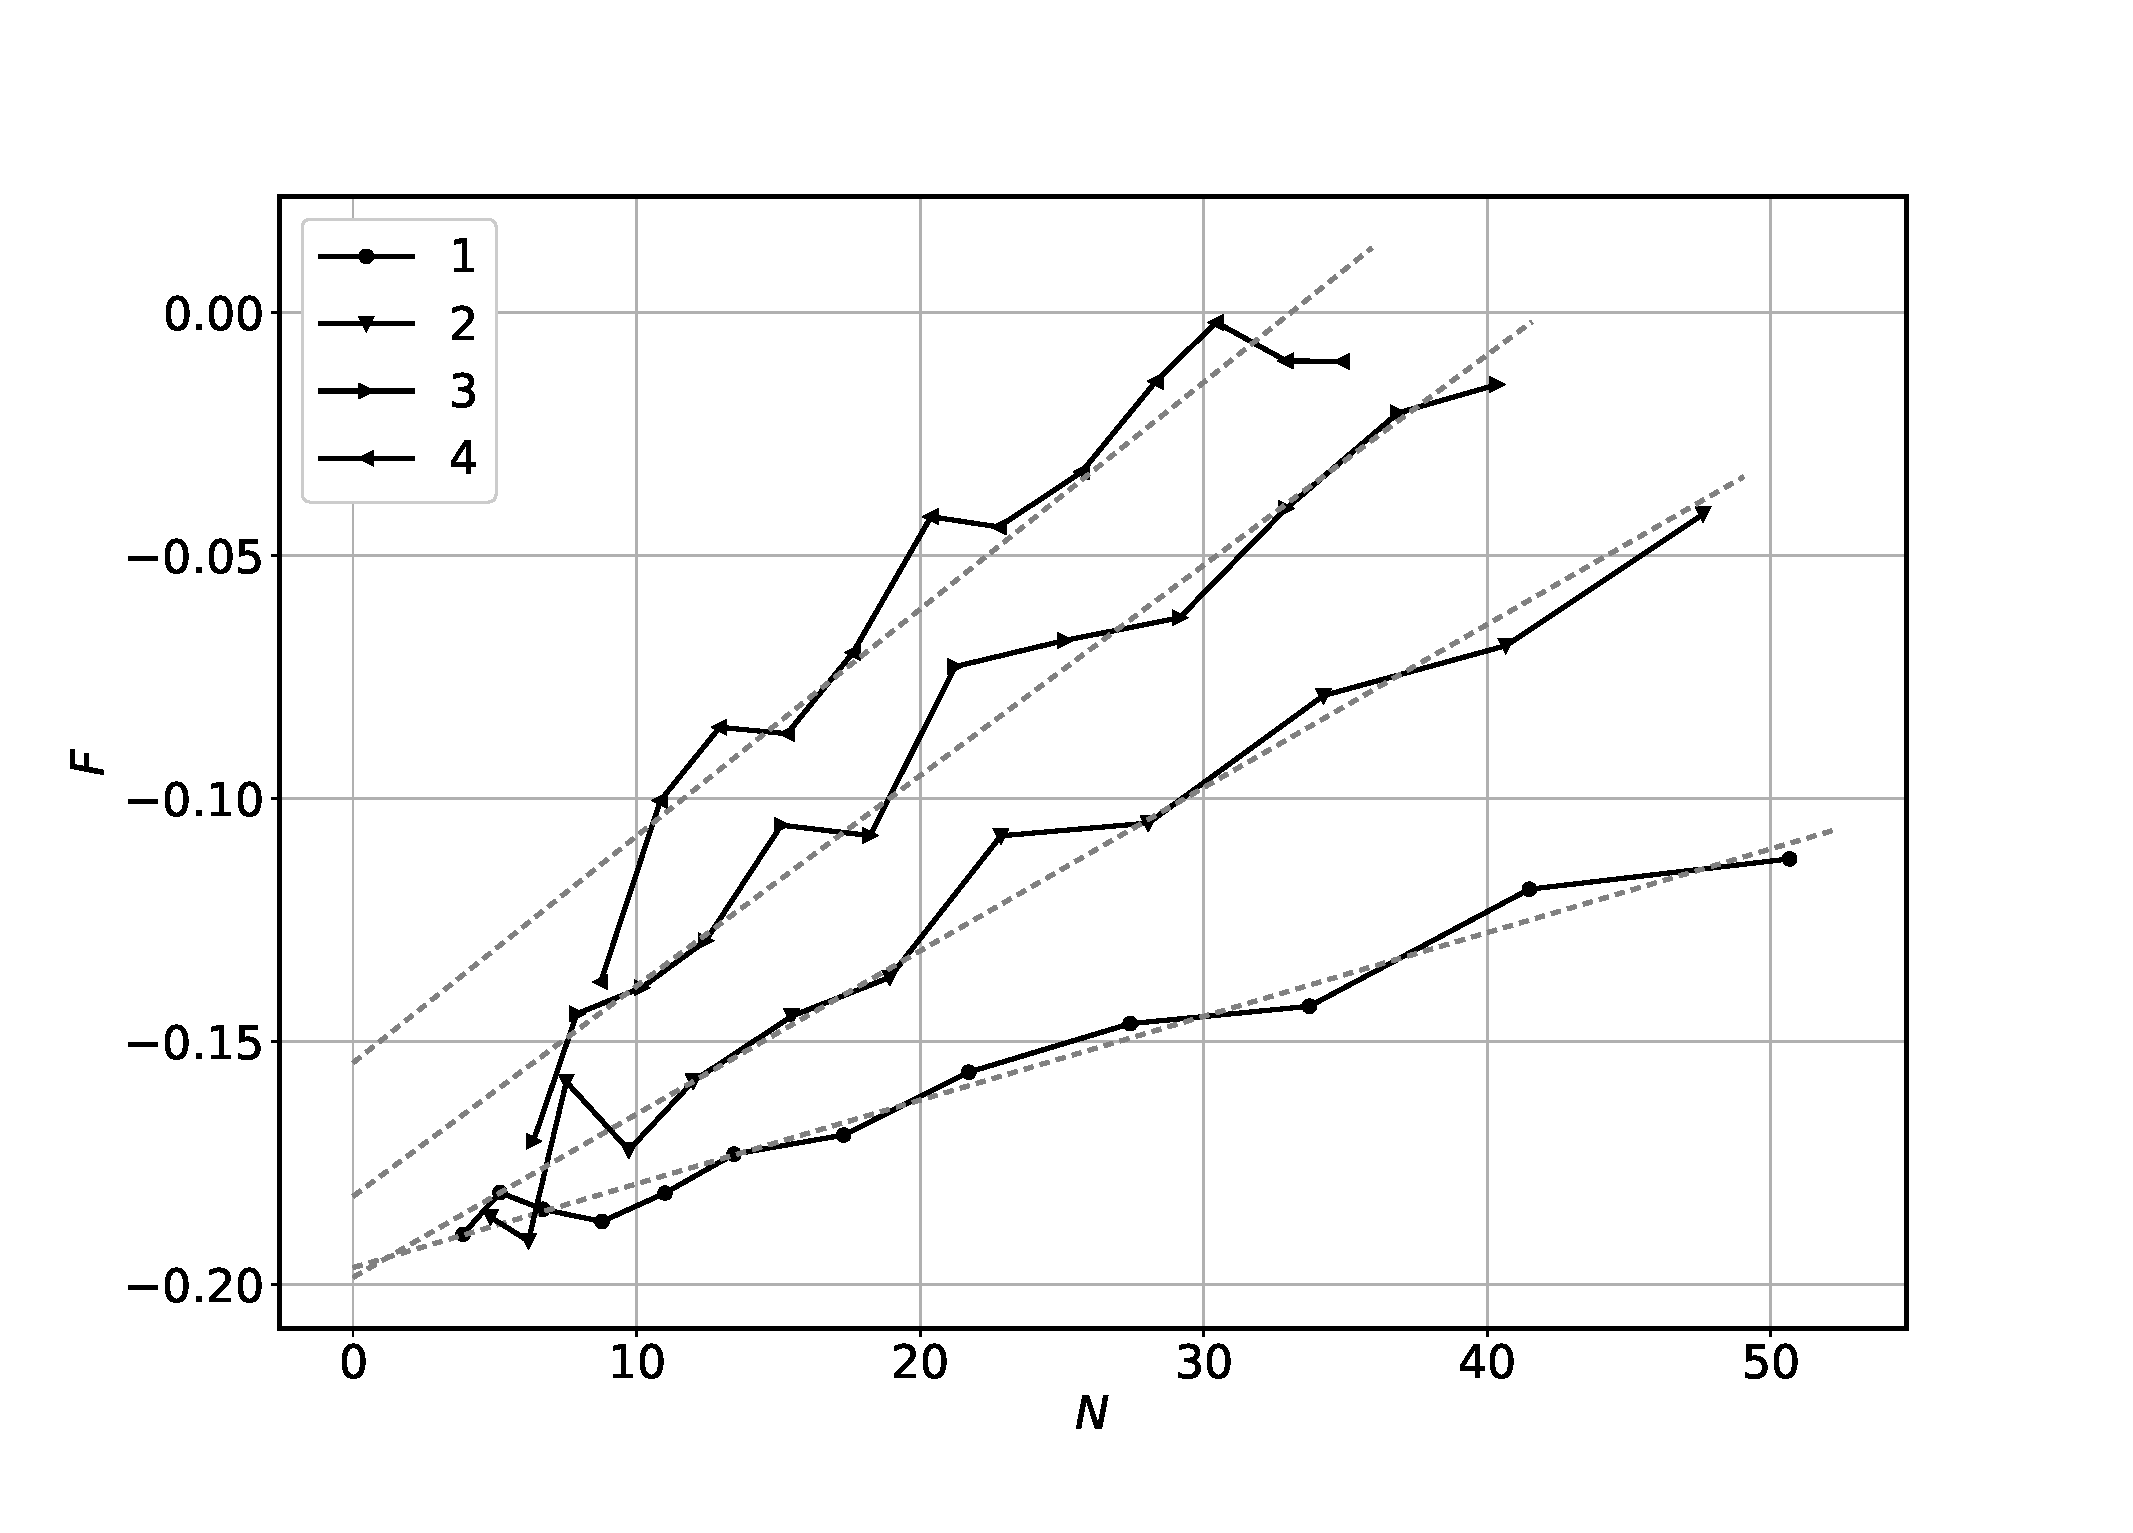
\includegraphics[width=0.75\textwidth]{FN.eps}
    \caption{Зависимость полной силы $F$ от количества частиц на единицу длины $N$, цифрами обозначены 
    измерения проводившиеся при соответствующих диаметрах частиц 1 - 5, 2 - 7, 3 - 9, 4 - 11.}
    \label{fig:FN}
\end{figure}

\begin{figure}[H]
    \centering
    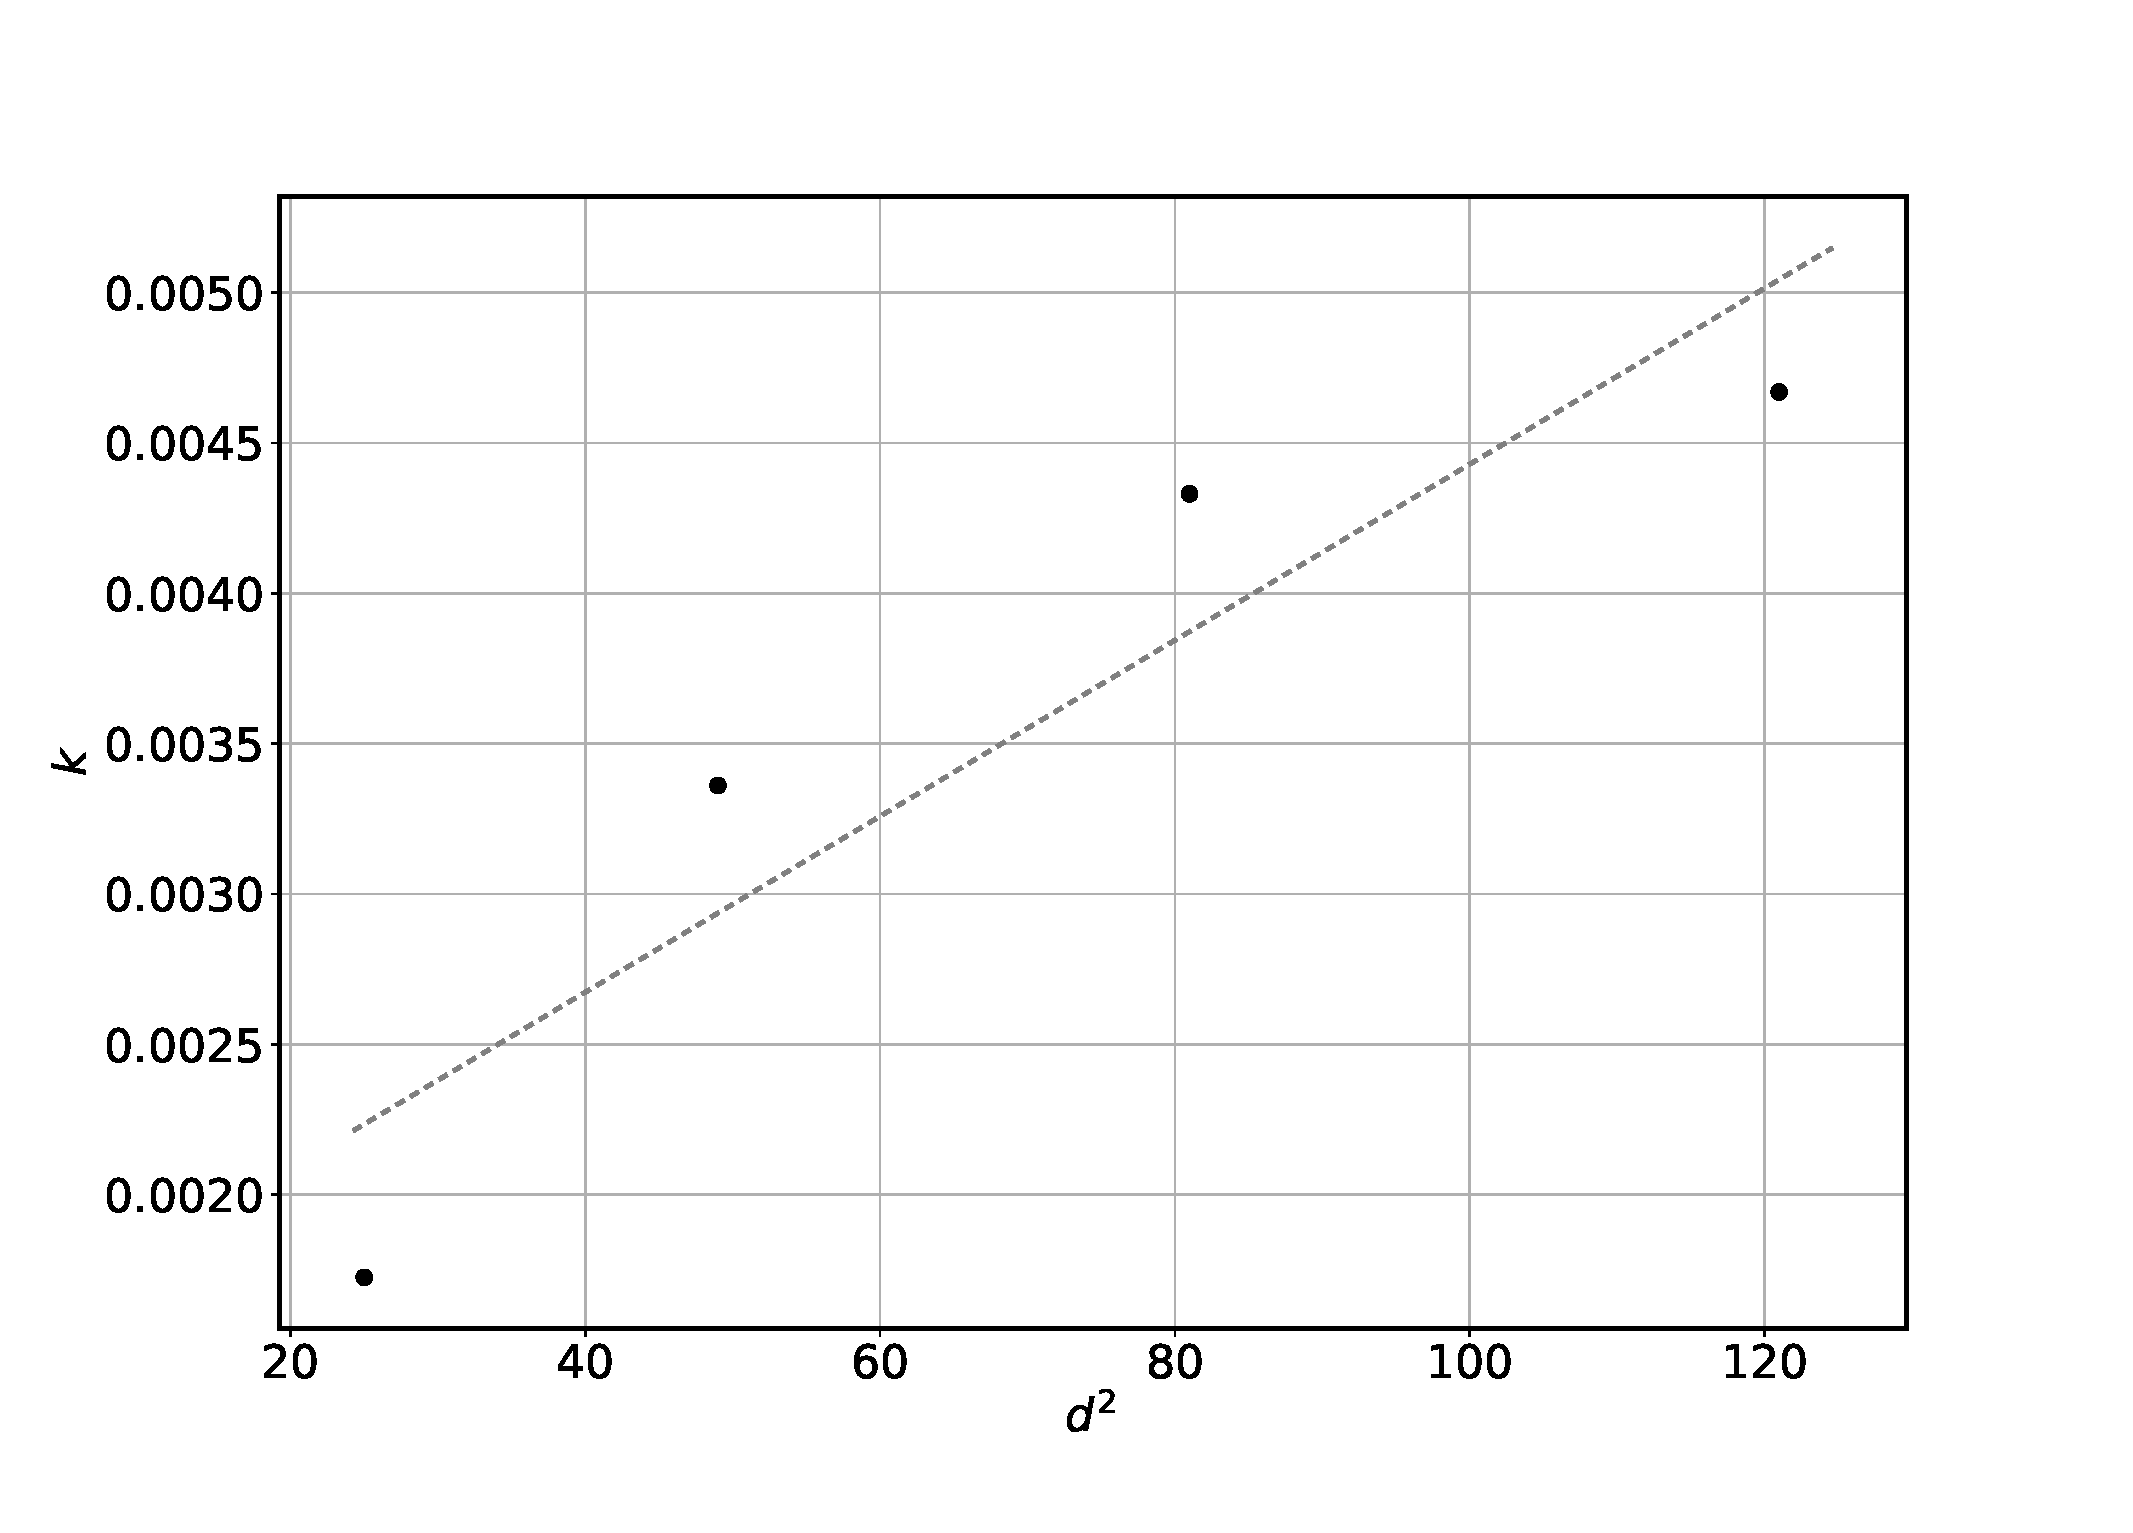
\includegraphics[width=0.75\textwidth]{kr.eps}
    \caption{Зависимость коэффициентов наклона $k = \frac{\partial F}{\partial N}$ от диаметра частицы в 
    квадрате $d^2$}
    \label{fig:kr}
\end{figure}

\section{Выводы}
В случае слабо-неидеальных газов сила Архимеда, действующая на отдельные молекулы не равна 0, а также 
зависит от типа слабо-неидеального газа. Для атомарных газов объяснить наличие силы Архимеда можно 
наличием области вокруг частицы, недоступной для других частиц. В таком случае сила Архимеда может быть зависана 
как 
\[
    F_a = pgV, 
\]
где $V$ - эффективный объём молекулы. Была получена оценка для эффективного объёма: 
\[
    V = 2b(T) = \frac{1}{2} \int \left( 1 - \exp \left\{ -\frac{U(r)}{kT} \right\}  \right)  \,\mathrm{d}V.
\] 
В случае плазмы эффективный объём будет зависеть не только от температуры, но также и от концентрации 
окружающих молекул, из-за этого зависимость силы архимеда не будет пропорциональна градиенту давлений. 
Численная оценка силы Архмеда для плазмы: 
\[
    F_a = -\frac{e^3}{2} \sqrt{\frac{\pi}{kTn^3}} \frac{dn}{dz} \left( \sum_{i=1} n_i z_i \right)^\frac{3}{2}.
\]

\section{Использованная литература}
\begin{thebibliography}{9}
    \bibitem{MainPaper}
    В.Л. Любошиц, М.И. Подгорецкий «О силе Архимеда, действующей на отдельные молекулы вещества во внешнем поле», 1991
    \bibitem{Kirichenko}
    Н.А. Кириченко «Термодинамика, статистическая и молекулярная физика»
    \bibitem{Landavsh}
    Ландау Л.Д., Лифшиц Е.М. «Статистическая физика»
\end{thebibliography}

\section{Приложения}
\subsection*{Вывод вириального разложения для атомарных газов} \label{app:1}
В случае неидеальных газов энергия системы складывается из энергии взаимодействия молекул и их кинетической энергии: 
\[
    E(p, q) = \sum_{i=1}^{N} \frac{{p_i}^2}{2m} + U.
\]
В данном выводе рассматривается одноатомный газ, потому потенциальная энергия взаимодействия является функцией взаимных расстояний атомов. 
Запишем статистическую сумму системы: 
\[
    Z = \int e^{-E(p, q)} \,\mathrm{d}p^3\mathrm{d}q^3 = 
    \int \exp {\left\{ \frac{-\sum_{i=1}^{N} \frac{{p_i}^2}{2m}}{kT} \right\} }  e^{-\frac{U}{kT}} \,\mathrm{d}p^3\mathrm{d}q^3 = 
    \int \exp {\left\{ \frac{-\sum_{i=1}^{N} \frac{{p_i}^2}{2m}}{kT} \right\} }  \,\mathrm{d}p^3 \int e^{-\frac{U}{kT}} \,\mathrm{d}q^3
\]
Первый интеграл совпадает с таковым для идеального газа. Предположим, что в один момент в газе сталкиваются не более одной пары атомов сразу.
Такое предположение не повлияет на общность рассуждений, так как свободная энергия аддитивна, и полученный 
результат можно обобщить на произвольный объём. В силу сделанных предположений энергию взаимодействия можно переписать как: 
\[
    U = \sum_{\alpha, \beta} U(r_\alpha - r_\beta) = \sum_{\alpha, \beta} U_{\alpha, \beta},   
\]
где суммирование производится по всевозможным парам атомов. 
Такая сумма отлична от 0 только в случае, если атомы находятся достаточно близко: 
\[
    e^{-\frac{U}{kT}} = \prod_{\alpha, \beta} e^{-\frac{U_{\alpha, \beta}}{kT}}.
\]
Введём функцию $f_{\alpha, \beta} = e^{-\frac{U_{\alpha, \beta}}{kT}} - 1$. И разложим произведение: 
\[
    \prod_{\alpha, \beta} \left( 1 + f_{\alpha, \beta} \right) = 1 + \sum_{\alpha, \beta} f_{\alpha, \beta} + \sum_{\alpha, \beta, \gamma} f_{\alpha, \beta} f_{\alpha, \gamma} + \dots   
\] 
Второе слагаемое отвечает за парное взаимодействие молекул, третье за тройное взаимодействие, и так далее. В нашем предположении 
ограничимся только первыми двумя слагаемыми. Тогда соответствующая статистическая сумма равна: 
\[
    Z_2 \approx \int \left( 1 + \sum_{\alpha, \beta} f_{\alpha, \beta} \right) \, \mathrm{d}q^3.
\]
Тогда так как энергия взаимодействия одинакова между любыми двумя атомами и зависит только от относительного расстояния перейдём к интегрированию только по одной координате: 
\[
    Z_2 = V^n + V^{n-1} \frac{N(N - 1)}{2} \int \left( e^{-\frac{U(r)}{kT}} - 1 \right) \,\mathrm{d}V.
\]
Тогда выразим свободную энергию газа: 
\[
    F = F_0 - T \ln \frac{Z_2}{V^n} = F_0 - T \ln \left( 1 + \frac{N^2}{2V} \int \left( e^{-\frac{U(r)}{kT}} - 1 \right) \,\mathrm{d}V \right) \approx 
    F_0 + \frac{N^2T}{V} b(T),  
\]
где $b(T) = \frac{1}{2} \int \left( 1 - e^{-\frac{U(r)}{kT}} \right) \,\mathrm{d}V$ - второй вириальный коэффициент.
Стоит отметить, что если $U(r)$ спадает с расстоянием медленней, чем $\frac{1}{r^3}$ интеграл не сойдётся, что означает 
непременимость модели для дальнодействующих потенциалов. 

\subsection*{Условие равновесия молекулы в гравитационном поле} \label{app:2}
Рассмотрим слой плотного вещества и для него запишем гидростатическое равенство: 
\[
    \frac{dP}{dz} = n f_z = -n \frac{du}{dz},
\]
где $u$ - потенциальная энергия отдельной молекулы.  
Тогда выразим $dP = -\frac{N}{V} du$ и подставим в выражение для дифференциала химического потенциала: 
\[
    d \mu = -s dT + \frac{V}{N} dP = -s dT - du \implies d (\mu + u) = -s dT. 
\]   
Так как система в равновесии, то температура постоянна, тогда выполнено 
\[
    d(\mu + u) = 0 \implies \mu + u = const.
\]
\subsection*{Вывод уравнения состояния классической плазмы} \label{app:3}
Рассмотрим полностью ионизированную плазму. Запишем несколько ключевых для решения выражений. 
Одно из них это электронейтральность плазмы: 
\[
    \sum_{i=1} z_i n_i, 
\]
где $z_i$ - зарядовое число $i$ сорта иона, $n_i$ - концентрация таких ионов в плазме. 
Основным предположением будет то, что энергия кулоновского взаимодействия много меньше кинетической энергии газа: 
\[
    n \propto \langle r \rangle^3 \ll \left( \frac{kT}{z^{2e^2} } \right)^3
\]
Запишем полную энергию взаимодействия ионов: 
\[
    E = \frac{1}{2} V \sum_{i=1} e z_i n_i \phi_i, 
\]
где $\phi_i$ - потенциал поля, действующего на ион $i$ сорта. 
В таком случае каждый ион создаёт вокруг себя заряженное ионное облако, 
концентрация ионов в нём подчиняется распределению Больцмана: 
\[
    n_i^{\prime} = n_i \exp \left( -\frac{z_i e \phi(r)}{kT} \right). 
\]
Коэффициент пропорциональности выбран равным $n_i$, так как при $r \to \infty$ концентрация должна сравняться 
с концентарцией всего газа. 
Тогда согласно уравнению Пуассона лаплассиан потенциала равен 
\[
    \triangle \phi = - 4\pi e \sum_{i} z_i n_i^{\prime}.
\]
В силу слабости электростатического взаимодействия разложим формулу для $n_i^{\prime}$ в ряд: 
\[
    n_a^{\prime} = n_a - n_a \frac{z_a e \phi}{kT}.
\] 
Введём переобозначение
\[
    \varkappa^2 = \frac{4\pi e^2}{kT} \sum_{i} n_i z_i^2
\] 
Тогда имеем уравнение: 
\[
    \triangle \phi - \varkappa^2 \phi = 0. 
\]
Ищем решение в виде $\phi = \frac{\xi}{r}$, лаплассиан примет вид: 
\[
    \triangle \phi = \frac{1}{r^2} \frac{\partial}{\partial r} r^2 \frac{\partial}{\partial r} \frac{\xi}{r} = \frac{1}{r^2} \frac{\partial}{\partial r} (r \xi^{\prime} - \xi) = \frac{\xi^{\prime\prime}}{r}. 
\] 
Подставив в исходное уравнение, получим: 
\[
    \xi^{\prime\prime} - \varkappa^2 \xi = 0,
\]
решением такого уравнения является затухающая экспонента: 
\[
    \phi = \frac{z_i e}{r} e^{-\varkappa r}.
\]
Полученный потенциал отвечает как потенциалу самого иона, так и ионного облака вокруг него.
Выделим дополнительный наведённый потенциал: 
\[
    \phi_i = \phi - \frac{e z_i}{r} = - e z_i \varkappa.
\]
Теперь подставим полученное значение потенциала в формулу для энергия взаимодействия: 
\[
    E = -\frac{V}{2} \varkappa e^2 \sum_{i} n_i z_i^2 = 
    -V e^3 \sqrt{\frac{\pi}{kT}} \left( \sum_{i} n_i z_i^2 \right)^\frac{3}{2}. 
\]
Для получения свободной энергии проинтегрируем соотношение 
$\frac{E}{T^2} = - \frac{\partial}{\partial T} \frac{F}{T}$: 
\[
    F = F_0 - \frac{2e^3}{3} \sqrt{\frac{\pi N^3}{kTV}}\left( \sum_{i=1} n_i z_i \right)^\frac{3}{2}.
\] 
\end{document}